\documentclass{beamer}
\usetheme{Madrid}

\usepackage[]{graphicx}
\usepackage{libertinus}
\usepackage[backend=biber]{biblatex}
\addbibresource{bibliography.bib}


\title{Untangling Knots Through Curve Repulsion}
\titlegraphic{
\includegraphics[height=2cm]{oxfordlogo.eps}}
\author{Joo-Hyun Paul Kim}

\begin{document}

% Title Page
\begin{frame}
    \titlepage
\end{frame}

\begin{frame}
    \frametitle{What the curious folks ponder about}
    \tableofcontents
\end{frame}

\section{Introduction}
\begin{frame}
    \frametitle{A Cool Knot}
    \begin{figure}[h]
        \centering
        \includegraphics[scale=0.25]{knot}
        \caption{Imagine your earphones getting tangled like this\ldots}
    \end{figure}

\end{frame}
\begin{frame}
    \frametitle{Aim}
    \begin{itemize}
        \item Finding homotopy from a knot to an unknot.
            \begin{figure}[h]
                \centering
                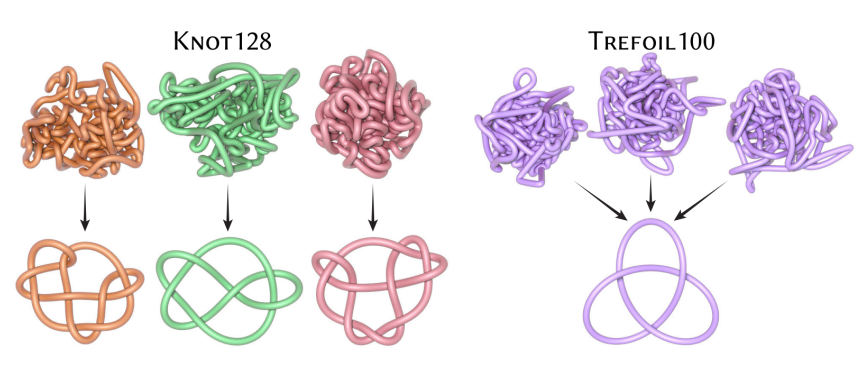
\includegraphics[scale=0.2]{knotsolving}
                \caption{Unknotting while avoiding self intersections.\cite{YSC2021}}
            \end{figure}
    \end{itemize}

\end{frame}

\begin{frame}
    \frametitle{Bibliography}
    \printbibliography
\end{frame}

\end{document}
